%% Based on a TeXnicCenter-Template by Tino Weinkauf.
%%%%%%%%%%%%%%%%%%%%%%%%%%%%%%%%%%%%%%%%%%%%%%%%%%%%%%%%%%%%%

%%%%%%%%%%%%%%%%%%%%%%%%%%%%%%%%%%%%%%%%%%%%%%%%%%%%%%%%%%%%%
%% HEADER
%%%%%%%%%%%%%%%%%%%%%%%%%%%%%%%%%%%%%%%%%%%%%%%%%%%%%%%%%%%%%
\documentclass[a4paper,oneside,10pt]{report}
% Alternative Options:
%	Paper Size: a4paper / a5paper / b5paper / letterpaper / legalpaper / executivepaper
% Duplex: oneside / twoside
% Base Font Size: 10pt / 11pt / 12pt


%% Language %%%%%%%%%%%%%%%%%%%%%%%%%%%%%%%%%%%%%%%%%%%%%%%%%
\usepackage[dutch]{babel} %francais, polish, spanish, ...
\usepackage[T1]{fontenc}
\usepackage[ansinew]{inputenc}

\usepackage{lmodern} %Type1-font for non-english texts and characters


%% Packages for Graphics & Figures %%%%%%%%%%%%%%%%%%%%%%%%%%
\usepackage{graphicx} %%For loading graphic files
%\usepackage{subfig} %%Subfigures inside a figure
%\usepackage{tikz} %%Generate vector graphics from within LaTeX

%% Please note:
%% Images can be included using \includegraphics{filename}
%% resp. using the dialog in the Insert menu.
%% 
%% The mode "LaTeX => PDF" allows the following formats:
%%   .jpg  .png  .pdf  .mps
%% 
%% The modes "LaTeX => DVI", "LaTeX => PS" und "LaTeX => PS => PDF"
%% allow the following formats:
%%   .eps  .ps  .bmp  .pict  .pntg


%% Math Packages %%%%%%%%%%%%%%%%%%%%%%%%%%%%%%%%%%%%%%%%%%%%
\usepackage{amsmath}
\usepackage{amsthm}
\usepackage{amsfonts}


%% Line Spacing %%%%%%%%%%%%%%%%%%%%%%%%%%%%%%%%%%%%%%%%%%%%%
%\usepackage{setspace}
%\singlespacing        %% 1-spacing (default)
%\onehalfspacing       %% 1,5-spacing
%\doublespacing        %% 2-spacing


%% Other Packages %%%%%%%%%%%%%%%%%%%%%%%%%%%%%%%%%%%%%%%%%%%
%\usepackage{a4wide} %%Smaller margins = more text per page.
%\usepackage{fancyhdr} %%Fancy headings
%\usepackage{longtable} %%For tables, that exceed one page


%%%%%%%%%%%%%%%%%%%%%%%%%%%%%%%%%%%%%%%%%%%%%%%%%%%%%%%%%%%%%
%% Remarks
%%%%%%%%%%%%%%%%%%%%%%%%%%%%%%%%%%%%%%%%%%%%%%%%%%%%%%%%%%%%%
%
% TODO:
% 1. Edit the used packages and their options (see above).
% 2. If you want, add a BibTeX-File to the project
%    (e.g., 'literature.bib').
% 3. Happy TeXing!
%
%%%%%%%%%%%%%%%%%%%%%%%%%%%%%%%%%%%%%%%%%%%%%%%%%%%%%%%%%%%%%

%%%%%%%%%%%%%%%%%%%%%%%%%%%%%%%%%%%%%%%%%%%%%%%%%%%%%%%%%%%%%
%% Options / Modifications
%%%%%%%%%%%%%%%%%%%%%%%%%%%%%%%%%%%%%%%%%%%%%%%%%%%%%%%%%%%%%

%\input{options} %You need a file 'options.tex' for this
%% ==> TeXnicCenter supplies some possible option files
%% ==> with its templates (File | New from Template...).



%%%%%%%%%%%%%%%%%%%%%%%%%%%%%%%%%%%%%%%%%%%%%%%%%%%%%%%%%%%%%
%% DOCUMENT
%%%%%%%%%%%%%%%%%%%%%%%%%%%%%%%%%%%%%%%%%%%%%%%%%%%%%%%%%%%%%
\begin{document}
\pagestyle{empty} %No headings for the first pages.


%% Title Page %%%%%%%%%%%%%%%%%%%%%%%%%%%%%%%%%%%%%%%%%%%%%%%
%% ==> Write your text here or include other files.
\begin{titlepage}

\begin{center}

%\vspace*{1cm}
\Large
\textsc{Universiteit van Groningen}\\

\vspace{5cm}

%\LARGE
\textsc{Gevorderde Algoritmen en Datastructuren\\[0.5\baselineskip]
door\\[0.5\baselineskip]
Jos van der Til \& Rene Zuidhof}\\

\vspace{5cm}
\textsc{\today}\\ %%Date - better you write it yourself.

\vspace{1cm}
\end{center}

\end{titlepage}

%% Inhaltsverzeichnis %%%%%%%%%%%%%%%%%%%%%%%%%%%%%%%%%%%%%%%
\tableofcontents %Table of contents
\cleardoublepage %The first chapter should start on an odd page.

\pagestyle{fancy} %Now display headings: headings / fancy / ...

%% Chapters %%%%%%%%%%%%%%%%%%%%%%%%%%%%%%%%%%%%%%%%%%%%%%%%%
%% ==> Write your text here or include other files.

%\input{intro} %You need a file 'intro.tex' for this.
\chapter{Introductie}

Dit verslag maakt deel uit van de cursus Gevorderde Algoritmen en Datastructuren van de Rijksuniversiteit Groningen. 
In dit verslag zal de tweede practicum opdracht behandeld worden. 
Deze opdracht omvat het vinden van een maximum flow in een flow network en de verschillende manieren, om dit te doen, te analyseren.

In hoofdstuk \ref{chap:maxFlowProblem} zal het probleem van het vinden van een maximum flow en het gebruikte algoritme beschreven worden. De hoofdstukken \ref{chap:depthfirst}, \ref{chap:breadthfirst} \& \ref{chap:priorityfirst} beschrijven de algoritmen die gebruikt worden om een pad te vinden door het netwerk. De conclusies van dit onderzoek staan in hoofdstuk \ref{chap:conclusion}.

Omdat het Ford-Fulkerson algoritme niet aangeeft op welke manier er een 'augmenting path' gevonden dient te worden, zijn er meerdere methodes beschikbaar.
De methodes die onderzocht zullen worden in dit document zijn:

\begin{enumerate}
	\item Depth-first search;
	\item Breadth-first search;
	\item Priority-first search.
\end{enumerate}

In het geval van een breadth-first search is het algoritme ook bekend als het Edmonds-Karp algoritme.
\chapter{Maximum flow probleem}
\label{chap:maxFlowProblem}
Om het probleem van het vinden van een maximum flow te kunnen begrijpen, volgt hier een korte introductie in de grafentheorie.

Een graaf is een verzameling punten (knopen) die verbonden zijn door lijnen (kanten). De kanten van een graaf kunnen een richting en/of een gewicht hebben. Een voorbeeld van een simpele graaf is te zien in figuur \ref{fig:6ngraph}.

\begin{figure}[h]
	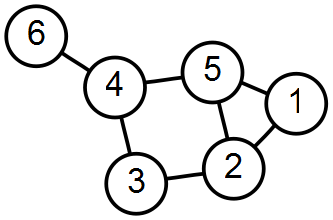
\includegraphics[width=0.5\linewidth]{maxflowproblem/6n-graph}
	\centering
	\caption{Een ongerichte en ongewogen graaf met 6 nodes}
	\label{fig:6ngraph}
\end{figure}

In figuur \ref{fig:flownetwork} is een voorbeeld van een flow network te zien. De flow in deze afbeelding is maximaal, immers de capaciteit van de beide kanten die leiden naar \textit{t} is volledig benut. Tevens te zien dat dit een gerichte (pijlen in plaats van lijnen als kanten) en gewogen (getallen bij de kanten) graaf is.

\begin{figure}[h]
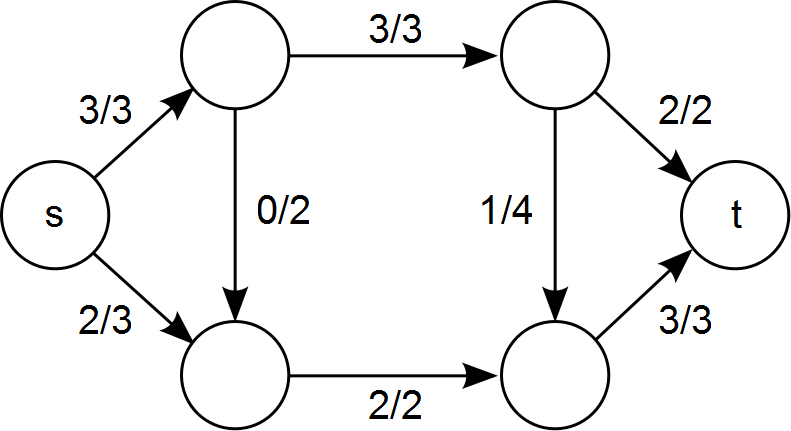
\includegraphics[width=0.5\linewidth]{maxflowproblem/max_flow}%
\centering
\caption{Voorbeeld van een flow netwerk met een maximum flow van \textit{s} naar \textit{t}. De getallen zijn flow / max capaciteit.}%
\label{fig:flownetwork}%
\end{figure}

Het probleem is nu om een flow te vinden van \textit{s} naar \textit{t} die maximaal is. Om dit op te lossen is er het Ford-Fulkerson algoritme, vernoemd naar L.R. Ford en D.R. Fulkerson die dit algoritme publiceerden in 1956. Deze wordt nader toegelicht in paragraaf \ref{sec:fordfulkerson}.

\section{Ford-Fulkerson algoritme}
\label{sec:fordfulkerson}

Het algoritme van Ford \& Fulkerson werkt eigenlijk volgens een heel simpel principe. Zolang er een pad is van \textit{s} naar \textit{t} met beschikbare capaciteit, dan wordt de flow daar langs gestuurd. Dit wordt herhaalt totdat er geen pad meer mogelijk is. Een pad van \textit{s} naar \textit{t} met beschikbare capaciteit wordt een 'augmenting path' genoemd.

De eisen die gesteld worden aan een geldige flow zijn:

\begin{itemize}
	\item De flow mag nooit groter zijn de de capacity van een kant. $0 \leq flow(u,v) \leq capacity(u,v)$
	\item De netto flow van een node is gelijk aan 0. Dit geldt niet voor \textit{s} of \textit{t}.$$\sum_{e \in E^-}\sum_{v \in E^+}{flow(e)-flow(v)} = 0$$
Waar $E^-$ de verzameling van uitgaande kanten is en $E^+$ de verzameling inkomende kanten van knoop $E$ is.
\end{itemize}

Omdat het Ford-Fulkerson algoritme niet aangeeft op welke manier er een 'augmenting path' gevonden dient te worden, zijn er meerdere methodes beschikbaar.
De methodes die onderzocht zullen worden in dit document zijn:

\begin{enumerate}
	\item Depth-first search;
	\item Breadth-first search;
	\item Priority-first search.
\end{enumerate}

\subsection{Pseudocode}

De pseudocode van het Ford-Fulkerson algoritme is te vinden in algoritme \ref{alg:FordFulkerson}.

\begin{algorithm}[h]
\caption{Ford-Fulkerson Algorithm}
\label{alg:FordFulkerson}
\begin{algorithmic}
\REQUIRE Input: Flow network $N$ containing graph $G$
\FORALL{edge $e \in N$}
 \STATE flow($e$) $\gets 0$
\ENDFOR

\STATE $stop \gets$ \FALSE

\REPEAT
\STATE traverse $G$ starting at $s$ to find an augmenting path to $t$ ($\pi$)

\IF{an augmenting path $\pi$ exists}

\STATE $\Delta \gets +\infty$

\FORALL{edge $e \in \pi$}
\IF{ residual capacity($e$) $\leq \Delta$}
\STATE $\Delta \gets $ residual capacity($e$)
\ENDIF
\ENDFOR

\FORALL{edge $e \in \pi$}

\IF{$e$ is a forward edge}
\STATE flow($e$) $\gets $ flow($e$) $+ \Delta$
\ELSE
\STATE flow($e$) $\gets $ flow($e$) $- \Delta$
\ENDIF

\ENDFOR

\ELSE
\STATE $stop \gets$ \TRUE
\ENDIF
\UNTIL{$stop$}

\end{algorithmic}
\end{algorithm}

\section{Analyse}

Voor de analyse van de zoekmethodes worden de grafen uit de figuren \ref{fig:analyseGraaf1} en \ref{fig:analyseGraaf2} gebruikt.
\begin{figure}[h]
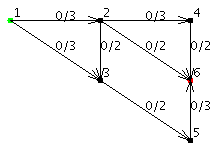
\includegraphics[width=\linewidth]{maxflowproblem/graph1}
\centering
\caption{Analyse graaf 1}
\label{fig:analyseGraaf1}
\end{figure}

\begin{figure}[h]
 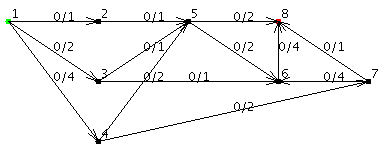
\includegraphics[width=\linewidth]{maxflowproblem/graph2}
\centering
\caption{Analyse graaf 2}
\label{fig:analyseGraaf2}
\end{figure}

\chapter{Depth-first search}
\label{chap:depthfirst}

De eerste methode die onderzocht is voor het zoeken naar een augmented path is de Depth-first search methode. Deze methode zal, zoals de naam suggereert, de diepte in gaan op zoek naar $t$. 


Tijdens het zoeken naar $t$ worden de edges gelabeld met $discovery$, $unexplored$ en $back$. 

\subsection{Pseudocode}
De pseudocode waar de code op gebaseerd is, is te vinden in algoritme \ref{alg:DFS}.

\begin{algorithm}[h]
\caption{Depth-first search Algorithm}
\label{alg:DFS}
\begin{algorithmic}
\REQUIRE Input: Graph g, Start vertex s, End vertex t, HashMap parents with vertexes and its parent edges
\STATE Label s as $EXPLORED$
\FORALL{edge $e \in s.incidentEdges$}
\IF e is not labeled as $UNEXPLORED$ && s.residualCapacity(e) > 0
\STATE w $\gets $ g.opposite(s, e)
\IF w is labeled as $UNEXPLORED$
\STATE label $e$ as $DISCOVERY$ edge
\STATE set $e$ as parent of $w$ in the hashmap parents
\STATE recursive call with g, w, t and parents
\ELSE
\STATE label $e$ as $BACK$ edge
\ENDIF
\ENDIF
\ENDFOR
\end{algorithmic}
\end{algorithm}

Wanneer het eindpunt $t$ bereikt is kan het algoritme stoppen. Nu kan met behulp van de $parents$ gezocht worden naar een pad van $s$ naar $t$ door te kijken wat de parent edge $e$ is van $t$. Nu zal gekeken worden naar de parent edge van de overstaande van $t$ via edge $e$. Door dit te doen tot er geen parent edge is zal $s$ bereikt worden.
\chapter{Breadth-first search}
\label{chap:breadthfirst}

De tweede manier om een augmenting path te vinden in een graaf is de breadth-first search. Deze methode, die ook gebruikt wordt in het Edmonds-Karp algoritme, vindt het kortste pad van $s$ naar $t$. Het kortste pad is in dit geval gedefineert als het pad met het laagste aantal kanten.

Het breadth-first doorlopen van een graaf is niet anders dan dat dat bij een tree gebeurt, elk niveau wordt volledig doorzocht, voordat het algoritme naar het niveau daar onder gaat. Dit is te zien in figuur \ref{fig:breadthFirstTree}, de getallen op de knopen geven aan in welke volgorde de boom doorzocht wordt.

\begin{figure}[h]
 \centering
 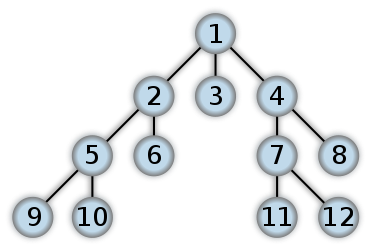
\includegraphics[width=0.5\linewidth]{breadthfirst/breadthfirsttree}
 \label{fig:breadthFirstTree}
 \caption{Breadth-first doorlopen van een boom}
\end{figure}

Om vervolgens het pad van $s$ naar $t$ te vinden in een graaf, wordt eerst de graaf doorlopen volgens het breadth-first principe totdat $t$ gevonden is. Terwijl de graaf doorlopen wordt, wordt bijgehouden welke kant leid naar welke knoop. Hierdoor is het gemakkelijk om het pad van $t$ naar $s$ terug te vinden. De pseudocode voor dit algoritme is te vinden in algoritme \ref{alg:breadthfirst}.

\section{Pseudocode}

\begin{algorithm}
 \caption{Breadth-first search path finding}
 \label{alg:breadthfirst}
 \begin{algorithmic}
  \REQUIRE \textbf{Input}: Graph G, Node s, Node t \\ 
\textbf{Output}: An augmenting path, or an empty path if none found.
  \STATE $Q \gets $ new queue
  \STATE $M \gets $ new hashmap
  \STATE $s$.state $\gets$ \textit{EXPLORED}
  \STATE $Q$.enqueue($s$)
  \WHILE{$\lnot Q$.isEmpty()}
   \STATE $v \gets Q$.dequeue()
   \FORALL{edge $e \in G$.incidentEdges($v$)}
    \IF{$e$.state = \textit{UNEXPLORED} $\land e$.residualCapacity() $ > 0$}
    \STATE $w \gets G$.opposite($v$, $e$)
    \IF{$\lnot w$.state = \textit{EXPLORED}}
      \STATE $Q$.enqueue($w$)
      \STATE $Q$.state = \textit{EXPLORED}
      \STATE $M$.put($w$, $e$) \COMMENT{$w$ discovered through edge $e$}
      \STATE $e$.state = \textit{DISCOVERY}
      \IF{$e$.start = $w$}
         \STATE Mark $e$ as forward
      \ELSE
         \STATE Mark $e$ as backward
      \ENDIF

      \IF{$w = t$}
         \STATE pathFound $\gets \FALSE$
         \STATE $p \gets w$
         \STATE $path \gets $ new list
         \WHILE{$\lnot$pathFound}
          \STATE $c \gets M$.get($p$) \COMMENT{Retreive edge $c$ that led to $p$}
          \STATE $path$.add($c$)      \COMMENT{Add edge $c$ to the path}
          \STATE $p \gets G$.opposite($p$, $c$) \COMMENT{ Go back another step in the graph}
          \IF{$p = s$}
            \STATE pathFound $\gets \TRUE$ \COMMENT{We found the start node, we are done.}
          \ENDIF
         \ENDWHILE
         \RETURN path
      \ENDIF
    \ENDIF
    \ELSE
      \STATE $e$.state $\gets$ \textit{BACKWARD}
    \ENDIF
   \ENDFOR
  \ENDWHILE
  \RETURN empty list \COMMENT{No path found}
 \end{algorithmic}
\end{algorithm}

\section{Analyse}
\chapter{Priority First Search}
\chapter{Conclusie}
\label{chap:conclusion}

%%%%%%%%%%%%%%%%%%%%%%%%%%%%%%%%%%%%%%%%%%%%%%%%%%%%%%%%%%%%%
%% BIBLIOGRAPHY AND OTHER LISTS
%%%%%%%%%%%%%%%%%%%%%%%%%%%%%%%%%%%%%%%%%%%%%%%%%%%%%%%%%%%%%
%% A small distance to the other stuff in the table of contents (toc)
\addtocontents{toc}{\protect\vspace*{\baselineskip}}

%% The List of Figures
\clearpage
\addcontentsline{toc}{chapter}{List of Figures}
\listoffigures

%% The List of Tables
\clearpage
\addcontentsline{toc}{chapter}{List of Tables}
\listoftables


%%%%%%%%%%%%%%%%%%%%%%%%%%%%%%%%%%%%%%%%%%%%%%%%%%%%%%%%%%%%%
%% APPENDICES
%%%%%%%%%%%%%%%%%%%%%%%%%%%%%%%%%%%%%%%%%%%%%%%%%%%%%%%%%%%%%
\appendix
%\input{FileName} %You need a file 'FileName.tex' for this.

\end{document}

